\chapter{Navegación semántica}
\label{cap:navegacionsemantica}
En este capítulo se expondrá una aplicación desarrollada para hacer uso todas las herramientas de las que hemos hablado anteriormente en el desarrollo del proyecto. Haremos uso del servidor de mapas dinámico, del paquete de localización AMCL y del paquete de navegación 
move\_base.

La aplicación se define como un sistema de navegación semántica o por etiquetas. Para ello se parte del mapa estático del escenario y se genera un nuevo mapa en el que se colorea cada estancia de la casa ,o cada \textit{waypoint} al que queremos que el robot navegue, con un tono de la escala de grises. Evitaremos coger el color negro, ya que está reservado para las paredes del mapa, y el color blanco que lo reservamos zonas que no queremos marcar. De esta manera podemos diferenciar fácilmente distintas estancias dentro de un mapa. 

\begin{figure} [hbtp]
  \begin{center}
    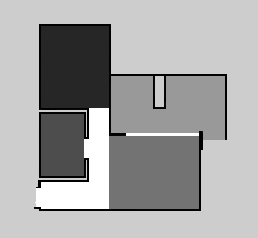
\includegraphics[width=7cm]{img/cap6/semanticmap}
  \end{center}
  \caption{Mapa semántico.}
  \label{fig:semanticmap}
\end{figure}

En un fichero de configuración, \textit{semantic\_navigation.yaml}, escribiremos el valor que corresponda a cada etiqueta y el destino al que queremos que el robot navegue cuando lancemos el paquete. El valor que le daremos será el correspondiente a la intensidad de gris de cada región, podemos obtenerlo fácilmente con una herramienta de edición de imágenes como por ejemplo \textit{gimp} y su herramienta \textit{recoge-color}.
\begin{lstlisting}[caption=Fichero de configuración de la navegación semántica, label={lst:semanticconfig}]
	kitchen: 60
	living_room: 45
	bathroom: 30
	principal_room: 15
	goal_place: principal room 
	# Options: principal room, bathroom, living room, kitchen
\end{lstlisting}

\begin{figure} [hbtp]
  \begin{center}
    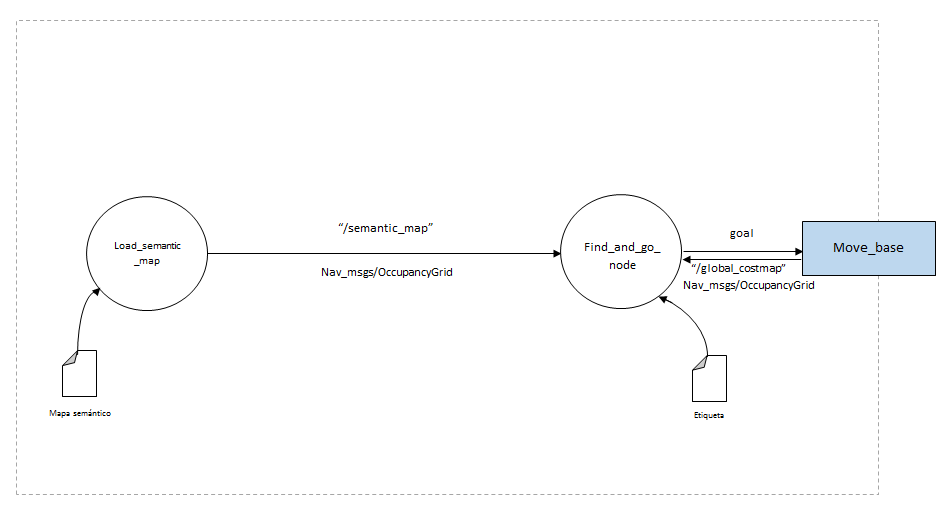
\includegraphics[width=18cm]{img/cap6/esquemasemantic}
  \end{center}
  \caption{Esquema del sistema de navegación semántica.}
  \label{fig:esquemasemantic}
\end{figure}

El esquema del sistema de navegación sigue la estructura de la figura xxx, en la que el nodo \textit{load\_semantic\_map\_node} carga desde fichero el mapa semántico y crea desde él un \textit{costmap} para poder ser analizado con mayor facilidad. 
Uno de los puntos fuertes del sistema es que siempre encontrará una celda libre que tomar como destino para enviársela a 
\textit{move\_base}. Esto es gracias a la composición del mapa semántico con el mapa que \textit{move\_base} genera a partir del mapa que le suministramos desde el servidor de mapas dinámico, figura \ref{fig:movebasemap}

\begin{figure} [H]
  \begin{center}
    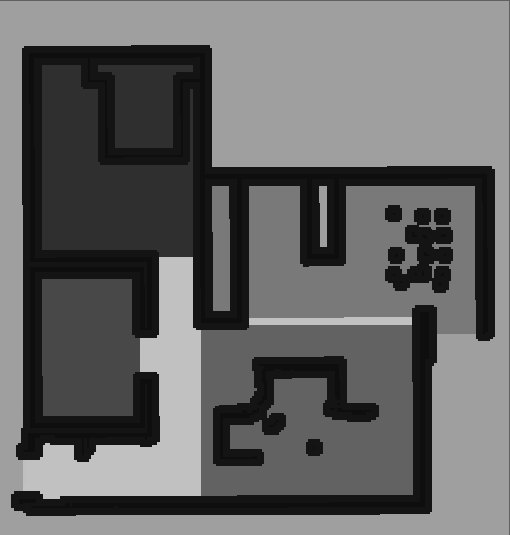
\includegraphics[width=7cm]{img/cap6/semanticmapcomp}
  \end{center}
  \caption{Composición del mapa semántico y mapa de move\_base.}
  \label{fig:semanticmapcomp}
\end{figure}

Usando esta composición nos aseguramos que el algoritmo que busca un punto que corresponda a la etiqueta que le hemos pasado no fije como destino un punto justo en la siguiente celda a una pared o a un mueble.